\chapter{Introduction}

Ability to track multiple objects simultaneously in real-time along with accurate (pixel-level) awareness for both stuff (background) and things (objects), are two of the fundamental vision-based challenges that modern autonomous and quasi-autonomous systems are faced with. We introduce two separate novel frameworks for both problems which improve on the current state-of-the-art and integrate them to form a joint ‘perception’ model capable of robust operation in object-dense and chaotic real-world scenarios.


\section{Problem and Scope}

\begin{figure*}[t]
\vspace{-0.7cm}
  \centering
  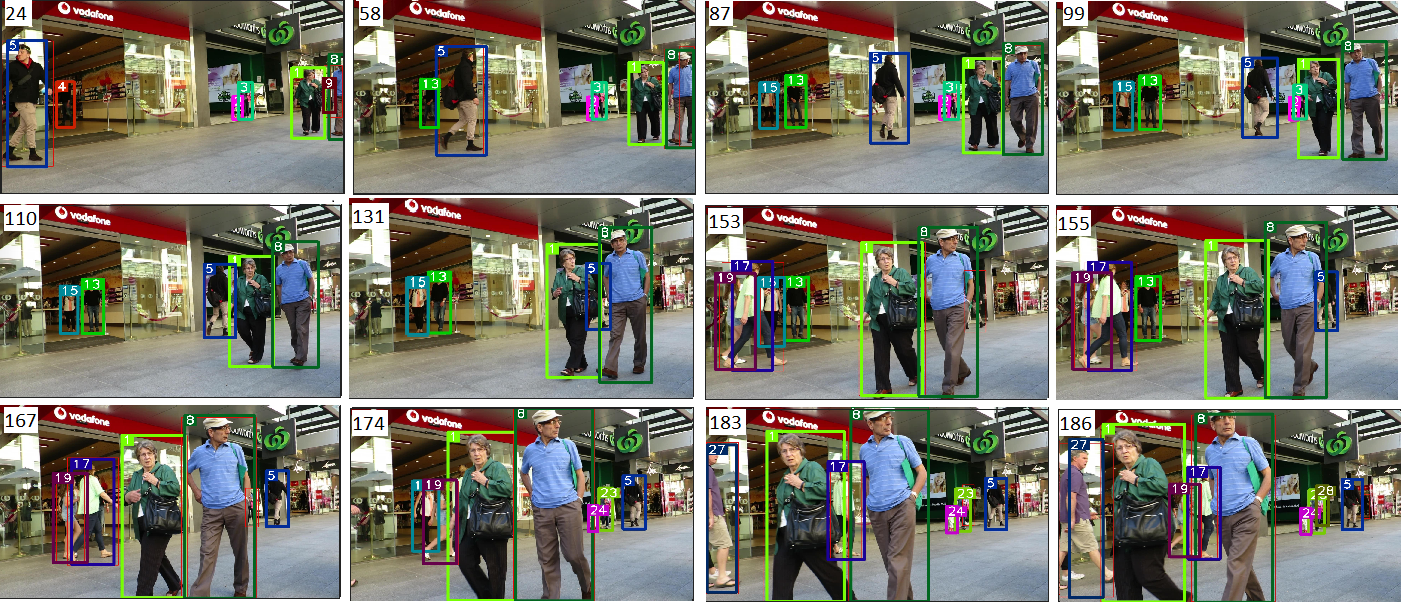
\includegraphics[ width=\textwidth]{figs/occlusions.png}
  \vspace{-0.5cm}
  \caption[Tracking Across Frames]{In the above diagram the numbers on the top left represent the frame number with detection bounding boxes in red and track bounding boxes in other colors. The above diagram depicts the occlusion handling done by our system. It can be seen that track 5(blue) observed in frame 24 is well tracked through out even after been occluded, given that the maximum occlusion duration is less than 30 frames. Additionally tracks 17 and 19 (blue and purple) are reidentified in frame 183 after been occluded. This is because, we control how much the occluding image’s features can affect the track’s template when the track is partially occluded}
  \label{fig:occlusions}
\vspace{1.0cm}
\end{figure*}

Multi-object tracking has been a critical and unavoidable problem even at the level of cutting edge technology. State of the art multi-object tracking systems are computationally heavy for the end devices whereas real time tracking systems are performing at the expense of accuracy and even highly accurate systems \cite{DeepSiam:deepSort} make errors in general and edge cases like occlusions, ego-motion, crossovers and rapid/random movements. The occlusions build up heavy risks in the automobile industry that looks forward for self driving cars. The inability to predict a pedestrian crossing behind the vehicle that slowed down on the side front or the incapability of the tracker to distinctly identify two persons at a point of crisscrossing can lead to critical issues in the field that is chaotic and requires memory other than detection for producing near intelligent results.

Most of the current systems are based on tracking through detection where the extensive development of efficiency and accuracy in state-of-the-art frame level detectors is used. The novel idea is to incorporate the temporal aspects into the algorithm due to the seemingly simple fact that objects do not disappear and should follow a time dependent progression within frame sequence given a satisfactory sampling rate in the sequence. Moreover, the improvement of depth sensation from both monocular and binocular image feeds \cite{DeepSiam:triangulation} and new methods of inverse perspective mapping  \cite{DeepSiam:perspective} build up the capacity to explore 3D tracking purely based on image data. This is important in the simultaneous localization of multiple real world objects with the observation of their dynamic aspects for decision making. 

Through this work we develop an online real-time multi-object tracking system for efficient human and vehicle tracking through the exploitation of appearance and spatiotemporal information through a novel Long and Short Term Memory (LSTM) \cite{DeepSiam:LSTM} based architecture along with the development of possible refinements to three dimensional track prediction through constraints observed in the Bird’s Eye View (BEV) space.

\begin{figure*}[t!]
\vspace{-0.5cm}
  \centering
  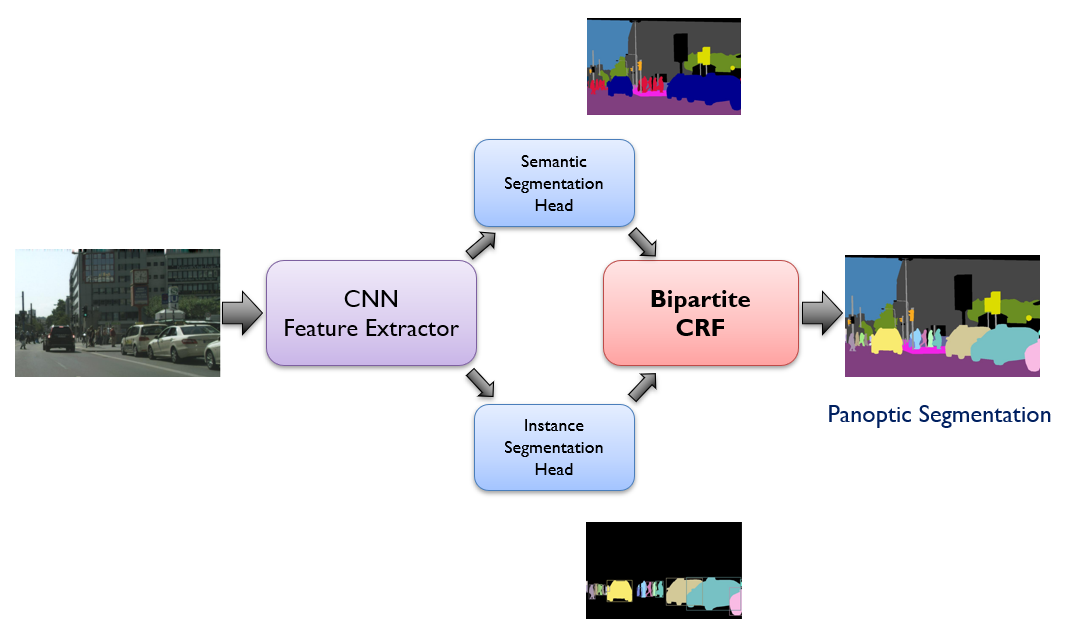
\includegraphics[trim = 1mm 1mm 1mm 1mm, clip, width=\textwidth]{figs/bcrf_arch.png}
  \vspace{-0.2cm}
  \caption[BCRF in an end-to-end trainable deep net]{{\bf BCRF in an end-to-end trainable deep net.} The Bipartite CRF proposed in this paper can be used to combine the predictions of a semantic segmentation model and an instance segmentation model to obtain a consistent panoptic segmentation.}
  \label{fig:bcrf_net}
\vspace{1.0cm}
\end{figure*}

Panoptic segmentation of images is a problem that has received considerable attention in computer vision recently. It combines two well-known computer vision tasks: semantic segmentation and instance segmentation. Panoptic segmentation differentiates between two types of semantic labels: \emph{stuff} labels and \emph{thing} labels. Stuff classes are semantic classes of shapeless regions of similar texture or material such as grass, sky, and road. Thing classes are semantic classes of countable objects such as people, animals, and vehicles~\cite{panoptickirillov2017}. The goal of panoptic segmentation is to assign a semantic label and an instance label for each pixel in the image. Clearly, the concept of instances is valid only for thing classes. Therefore, the instance label of a pixel labeled with a stuff semantic class is neglected.

Although semantic segmentation and instance segmentation are apparently very related problems, in the current state of the art methods in computer vision, they are solved in substantially different ways. The semantic segmentation problem is usually solved with a fully convolutional network architecture such as FCN~\cite{fcn_pami2017} or DeepLab~\cite{Deeplab_pami}, whereas the instance segmentation problem is solved using an object detector based method such as Mask-RCNN~\cite{mask_rcnn}. Each of these architectures have their own strengths and weaknesses. For example, fully-convolutional network based semantic segmentation methods have a wide field of view, specially when used with dilated convolutions~\cite{dialated_conv}, and therefore can make semantic segmentation predictions with global information about the image. In contrast, region proposal based networks, such as Mask-RCNN, focus on specific regions of interest during the later stages of the network and make predictions using strong local features available within a given region of interest. It is natural to think of a systematic way of combining the complementary strengths of these two different approaches.

We propose a Conditional Random Field (CRF) based framework for panoptic segmentation. Our framework, named Bipartite Conditional Random Fields (BCRF), takes inputs from both a semantic segmentation module and an instance segmentation module, and uses additional prior ideas about a good panoptic segmentation. It then performs probabilistic inference on a graphical model to obtain the best panoptic label assignment given the semantic segmentation classifier, the instance segmentation classifier, and the image itself. Our framework provides a heuristic-free, probabilistic method to combine semantic segmentation results and instance segmentation results - yielding a panoptic segmentation with consistent labeling across the whole image. We formulate our bipartite CRF using different energy functions to encourage the spatial, appearance and semantic consistency of the final panoptic segmentation. The optimal labeling is then obtained by performing mean field inference on the bipartite CRF - solving for both the semantic segmentation and the instance segmentation in a jointly optimal way.

Importantly, we show that our proposed BCRF inference is fully differentiable with respect to the various parameters used within the CRF and also the semantic segmentation and instance segmentation classifier inputs. Therefore, the BCRF module can be used as a first-class citizen of a deep neural network to perform panoptic segmentation. A deep network equipped with the BCRF module is capable of structured prediction of consistent panoptic labels and is end-to-end trainable. We show an example application of this framework and demonstrate that superior results can be used by probabilistic combination of a semantic segmentation classifier and an instance segmentation classifier in the BCRF framework.



\section{Related Work}

\subsection{Single Frame Detectors}

A considerable number of new network architectures have been developed for object detection and classification where growth in accuracy and speed had been the key goals. Out of the main state-of-the-art systems, the models based on Faster-RCNN \cite{DeepSiam:FasterRCNN} that had been developed from Fast RCNN \cite{DeepSiam:FastRCNN} use a Region of Interest (RoI) to detect the objects and found to be highly accurate through the improvements with introduction of Region Proposal Network (Fully Convolutional Network that proposes regions). The single stage detectors like YOLO \cite{DeepSiam:YOLO} (You Only Look Once) network on the other hand have been optimized for speed over accuracy. They explore the entire image as a whole grid instead of computing regions of interest and can achieve high performance in frame rate (exceeding 45fps). For the industry of self driving vehicles and the real-time automated market background both accuracy and speed are crucial. A notable aspect that each architecture has adopted to improve performance is approaching localization of an anchor-based classification task followed by regression as opposed to a purely regression task. This idea will serve as one of the baselines for our work.

\subsection{Single Object Trackers}

Tracking algorithms move for deep architectures (ex: Fully Convolutional Siamese) that use deep similarity learning for tracking \cite{DeepSiam:SiamFC, DeepSiam:siammask} to solve the key challenges of changes in lighting conditions, orientation and viewpoint. Extension of these methods to the multi-object setting is yet to be achieved. Further, some algorithms have been designed to learn online to track generic objects. However, learning online needs higher computational capacity at the end device which is not a luxury that could be afforded. The work by David Held et al. on GOTURN i.e. Generic Object Tracking Using Regression Networks \cite{DeepSiam:100fps} depict the capability of achieving 100fps at test time with frozen weights. But their work is limited to single object tracking.

\subsection{Joint Tracking and Detection}

The novel idea in tracking and video recognition is the ability of improving the detection and tracking inter-dependently. That is to enhance the detection using temporal information and improve the track using both detection as well as temporal information. There has been significant progress in this area too \cite{DeepSiam:Tracktodetect, DeepSiam:mobvid}. Tracking by detection had been a considerably successful topic in the field, but this aggregation of the temporal information has turned the efforts to a different path of exploration that could predict the next level of action which is steps beyond ordinary tracking. The common idea behind these methods is the usage of temporally aware feature maps for tackling the task of detection. The key shortcoming is the lack of direct track outputs which are a requirement for tracking. 

\subsection{Multi-Object Trackers}

SORT (Simple Online and Real Time Tracking \cite{DeepSiam:Sort}) with a deep association metric \cite{DeepSiam:deepSort} presents an implementation of the Kalman filter for exploiting the temporal information and a neural network incorporating the detections and deep appearance descriptor. The key challenge faced by this work is its failure to tackle crossovers, occlusions, and modeling non-linear object motion. Improvement of the temporal aspect using the LSTMs in single object setting \cite{DeepSiam:multitarget} has presented promising results in catering to these problems. Further, the possibility of data association of random cardinality, specifically through the birth and death of characters (track initiation and termination) using LSTMs alone \cite{DeepSiam:multitarget} is equally promising. The exploitation of multiple fields of view by relating deeper layers in Siamese networks \cite{DeepSiam:multicontext} show the potential of Siamese matching even though it is considerably inhibited by the scenarios that have occlusions.

\subsection{BEV space and 3D tracking}

The methods for inverse perspective mapping and 3D detection have been extensively researched as means of depth sensation through both monocular \cite{DeepSiam:triangulation, DeepSiam:perspective} and binocular \cite{DeepSiam:triangulation} image feeds. The achievement of accuracy in depth sensation through images has approached the level of expensive range sensor data to a considerable extent. However, the task of 3D tracking is currently dominated by the algorithms that run on range sensor information \cite{DeepSiam:fastandfurious}.


\subsection{Panoptic Segmentation}

The task of semantic segmentation has historically captured much attention~\cite{semantic01, semantic02, semantic03, pasvalVOC2014} with multiple innovations emerging as a direct result~\cite{FCN_2015, Badrinarayanan2017SegNetAD, scaleAwareSemantic}. With the popularity of deep convolutional feature extractors, multiple recent works have focused on multi-scale feature extraction~\cite{Zhao2016PyramidSP, scaleAwareSemantic, dialated_conv, Yu2017DilatedRN} and end-to-end structured predictions~\cite{Zhen_ICCV15_CRFRNN, Deeplab_pami, Chen2014SemanticIS, Arnab_arxiv2015, Liu_2015_ICCV, Chen2017RethinkingAC} to better solve this task. While the former allows networks to capture objects of all scales, the latter allows better granularity in outputs. Further, the wider field of view in these networks, especially since the introduction of dilated convolutions~\cite{dialated_conv, Yu2017DilatedRN}, provides better contextual understanding that directly benefits the task of semantic segmentation. This greater awareness of global information is a key uniqueness of most recent works. Also note how multiple approaches based on structured predictions~\cite{Zhen_ICCV15_CRFRNN, Liu_2015_ICCV, Arnab_arxiv2015, refine_net} have been highly successful in the task of semantic segmentation. 

Along with the emergence of high accurate object detection works~\cite{faster_rcnn, ssd_paper}, instance specific semantic segmentation started gaining significant attention. Early approaches use structured prediction based methodologies~\cite{early_instance_seg, DPM}, some often involving CRFs~\cite{instanceCRF01, instanceCRF02}. With the advent of deep learning based approaches, instance segmentation methodologies have mostly taken the form of two-stage proposal based approaches~\cite{earlyInstance01, SelectiveSearch, earlyInstance02, instanceFCN01}. These methods were superseded by Mask R-CNN~\cite{mask_rcnn}, laying the foundation for most current state-of-the-art instance segmentation approaches. Mask R-CNN builds off a conceptually simple extension of Faster R-CNN~\cite{faster_rcnn} obtained by adding a separate object mask prediction branch in parallel to the existing ones, capturing information local to each instance. This key contrasting feature is common even in later works built off Mask R-CNN~\cite{instance_path}. Another similar recent work by Arnab \emph{et al.}~\cite{Anurag17} moves in a slightly new direction by using a CRF to obtain instance segmentation outputs from a semantic segmentation using bounding box (from an object detection network) and instance shape cues. Our work differs from this in three significant ways: presence of pixel-wise cross potentials, using instance mask cues from a region-based network, and the ability to explicitly learn and model relationships between classes. 

Since its formal introduction by Kirillov \emph{et al.}~\cite{panoptickirillov2017}, the task of panoptic segmentation has gained popularity, with multiple works attempting to transform existing network architectures to tackle this task~\cite{panoptic_spatial_ranking, panoptic_DeeperLab, panoptic_SSAP, panoptic_attention, panoptic_scene, Upsnet_paper}. A key feature common among most of these works is fusing the logit outputs of existing semantic and instance segmentation networks to obtain a panoptic segmentation using some unique approach. The work of Arnab \emph{et al.}~\cite{Anurag17} which emerged prior to this, may also be considered as an initial step in this direction. The work by Kirillov \emph{et al.}~\cite{panoptics_fpn} explores extending a feature pyramid network ~\cite{FPN_paper} based Mask R-CNN ~\cite{mask_rcnn} to output semantic segmentation as well, followed by heuristic based fusion to produce a panoptic output. Another similar approach is seen in the work by Xiong \emph{et al.}~\cite{Upsnet_paper} where the outputs are combined using a simple resizing and addition of semantic and instance logits alongside a method to output additional unknown labels for difficult pixels. Our work differs from these approaches with the inclusion of a CRF based layer for combining the two semantic and instance heads. 


\subsection{Conditional Random Fields}

Conditional Random Fields (CRFs) are known as excellent models for structured prediction tasks such as semantic segmentation. Early works that used CRFs for semantic image segmentation includes ~\cite{instanceCRF01, instanceCRF02}. Most of these early methods of CRFs for semantic segmentation used 4-connected or 8-connected locally connected graphs. In~\cite{densecrf}, the authors proposed an efficient mean field based inference algorithm to solve fully connected CRFs with Gaussian edge potentials. The authors of~\cite{Zhen_ICCV15_CRFRNN} later showed that this CRF inference algorithm can be formulated as a Recurrent Neural Network (RNN). This module, known as CRF-RNN, was plugged into a fully convolutional network to obtain the state-of-the-art in semantic image segmentation at the time. Similar trainable CRF models have been used in works such as \cite{arnab_eccv_2016}, for semantic segmentation with higher-order potentials and,~\cite{Anurag17} for instance segmentation. In~\cite{li_eccv_2018}, where the problem of panoptic segmentation with weak and semi supervision was addressed, the authors used a CRF for refining instance segmentation labels. However, it worked on homogeneous instance labels only and therefore was similar in spirit to previous fully connected CRFs.

In our work, we propose a bipartite CRF operating on the semantic segmentation task and the instance segmentation task \emph{simultaneously}. This CRF has energies within semantic segmentation labels, energies within instance segmentation labels, and also energies \emph{across} semantic and instance segmentation labels. To the best of our knowledge, this is the first time a bipartite CRF with cross connections between semantic and instance labels has been proposed in the context of pixel-wise labeling.

\section{Method of Investigation}
 Primary objective is to develop a system for real-time multi-object tracking and segmentation through a novel architecture. This includes having the ability to model the complex stochastic environments in details pertaining to spatiotemporal aspects, class wise and object wise relations and have confident as well as precise throughput that matches the current state-of-the-art system designs. 
 
 The first most approach is the replication of current state of the art systems that have similar approaches and producing the results as per their description followed by the integration of our methodology (described in the next chapter) for improvement analysis through ablation studies and moving towards a coherent system following the requirements specified in problem statement. Due to the fact that approach considered is a research based method, extensive experiments were carried out for modular development and testing on public standard datasets. 
 
 
\section{Principal Results of Investigation}
The investigation on the multi-object tracker paved the way for developing a tracking network that process both appearance information as well as temporal information on the video feeds in real time. The investigation showed the capability of novel Long Short Term Memory (LSTM) modules to robustly adjust to the temporal information and predict the bounding box locations in the extrapolated frames of a given video (or an image sequence). Furthermore, the experiments done on the association of data and related predictions revealed the extents to which the novel network could be expanded and possible limitations (explained in chapters \ref{chapter:method} and \ref{chapter:results}).

The segmentation task revealed the capability of the Bipartite Conditional Random Field to behave as a module (a single layer that can be plugged to any deep network for information integration) that provides a probabilistic matching for panoptic segmentation of the images. The system was tested on datasets and compared to the outputs for current state of the art systems and revealed that novel methodology works in par with results of most approaches and can also surpass their results when architectures with bipartite heads are integrated with our layer which also presents a significant visual development and smoothening.  